\documentclass[tikz,border=10pt]{standalone}
\usepackage{tikz}
\usetikzlibrary{shapes.geometric, arrows.meta, positioning, calc, shadows}

\begin{document}

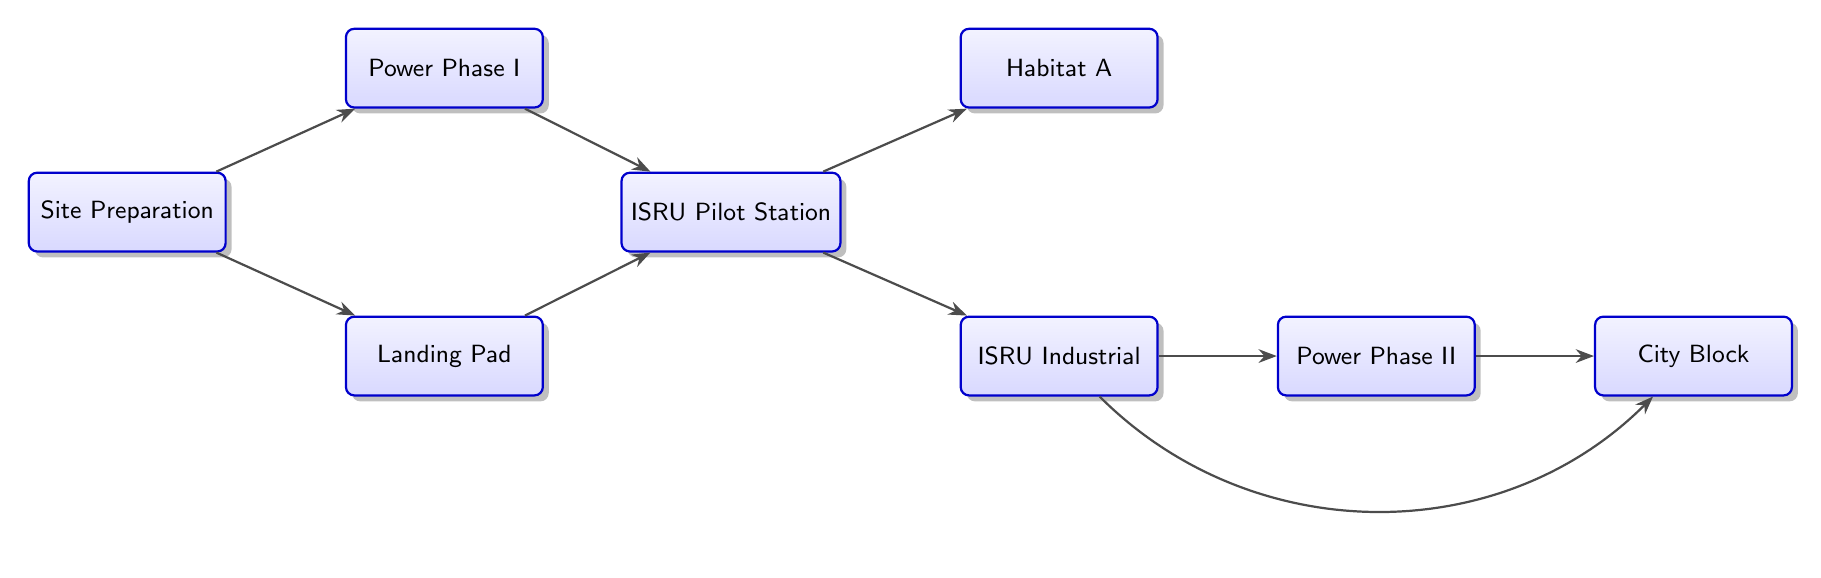
\begin{tikzpicture}[
    node distance=1.0cm and 1.5cm,
    every node/.style={font=\sffamily\small},
    task/.style={
        rectangle, 
        rounded corners=3pt, 
        minimum width=2.5cm, 
        minimum height=1cm, 
        text centered, 
        draw=blue!80!black, 
        top color=blue!5,
        bottom color=blue!15,
        thick,
        drop shadow
    },
    arrow/.style={thick, ->, >=Stealth, color=gray!60!black}
]

    % Define nodes
    \node (prep) [task] {Site Preparation};
    
    \node (u_power) [task, above right=0.8cm and 1.5cm of prep] {Power Phase I};
    \node (landing) [task, below right=0.8cm and 1.5cm of prep] {Landing Pad};
    
    % Pilot depends on u_power and landing
    % Position it to the right of the midpoint
    \node (pilot) [task, right=5cm of prep] {ISRU Pilot Station};
    
    \node (hab) [task, above right=0.8cm and 1.5cm of pilot] {Habitat A};
    \node (ind) [task, below right=0.8cm and 1.5cm of pilot] {ISRU Industrial};
    
    \node (d_power) [task, right=1.5cm of ind] {Power Phase II};
    
    % City Block depends on d_power and ind (redundant since d_power depends on ind)
    % Position it to the right of d_power, maybe centered between d_power level and something else?
    % Just flow linearly from d_power is fine.
    \node (city) [task, right=1.5cm of d_power] {City Block};

    % Draw connections
    \draw [arrow] (prep) -- (u_power);
    \draw [arrow] (prep) -- (landing);
    
    \draw [arrow] (u_power) -- (pilot);
    \draw [arrow] (landing) -- (pilot);
    
    \draw [arrow] (pilot) -- (hab);
    \draw [arrow] (pilot) -- (ind);
    
    \draw [arrow] (ind) -- (d_power);
    
    % Two inputs to city: from d_power and from ind.
    % Draw ind->city curved since d_power is in between?
    % Or note that T06->T08 is technically redundant if T06->T07->T08 exists.
    % However, if we want to show it explicitly:
    \draw [arrow] (d_power) -- (city);
    \draw [arrow] (ind) to[bend right=45] (city); 

\end{tikzpicture}

\end{document}
